\documentclass[16pt]{beamer}
\usepackage[utf8]{inputenc}

\title{Réseaux sociaux, aspirateurs de données}

\usetheme{default}

\usepackage[utf8]{inputenc}
\usepackage{amsmath}
\usepackage{amsfonts}
\usepackage{amssymb}
\usepackage{pgf}
\usepackage{color}
\usepackage[frenchb]{babel}
\usepackage{amssymb}
\usepackage{hyperref}

\usefonttheme{default}
\usepackage{DejaVuSans}
%\usepackage[sfdefault]{FiraSans} %% option 'sfdefault' activates Fira Sans as the default text font
\usepackage[T1]{fontenc}
\renewcommand*\oldstylenums[1]{{\firaoldstyle #1}}


\setbeamertemplate{navigation symbols}{} %remove navigation symbols

\author{Cédric Jeanneret (aka \href{https://www.twitter.com/SwissTengu}{@SwissTengu})}
\institute{\href{https://www.ethack.org/}{EthACK.org}}
\date{\today}

\definecolor{linecolor}{HTML}{4d4c4c}

\setbeamercolor{linecolor}{fg=white,bg=linecolor}

\setbeamertemplate{headline} {
	\begin{beamercolorbox}[wd=\paperwidth,dp=8pt,ht=12pt,leftskip=.29cm,rightskip=.29cm]{linecolor}
	\hfill
	\hypersetup{
		colorlinks=true,
		linkcolor=white,
		urlcolor=white,
	}
	\insertinstitute
	\end{beamercolorbox}%
}

\setbeamertemplate{footline}{%
	\begin{beamercolorbox}[wd=\paperwidth,dp=9pt,ht=0.4cm,leftskip=.29cm,rightskip=.3cm]{linecolor}
	\pgfputat{\pgfxy(0.455,-0.315)}{\pgfbox[center,base]{
\includegraphics[width=1.5cm]{../common/logo_537.png}}}
	\hfill
	\inserttitle
	\end{beamercolorbox}%
}


\hypersetup{
	colorlinks=true,
	linkcolor=blue,
	urlcolor=blue,
	pdfborderstyle={/S/U/W 1},
	pdfborder=0 0 1,
	linkbordercolor={0 0 0},
	urlbordercolor={0 0 0},
}


\begin{document}

{
\setbeamertemplate{footline}{%
	\begin{beamercolorbox}[wd=\paperwidth,dp=8pt,ht=12pt,leftskip=.29cm,rightskip=.3cm]{linecolor}
	\hfill
	\inserttitle
	\end{beamercolorbox}%
}

% center first slide — not a title, but almost
{
\centering
\begin{frame}

EthACK
\vspace{0.5cm}

The Swiss Privacy Basecamp 
\vspace{0.5cm}


\includegraphics[width=4cm]{../common/logo_537.png}

\end{frame}
}
}

\begin{frame}{EthACK ?}
\begin{itemize}
	\item Éthique
	\item État
	\item ACKnowledgement (reconnaissance)
	\item Hacking (éthique, évidemment)
	\item …
\end{itemize}
\end{frame}

\begin{frame}{Pourquoi ?}
\begin{itemize}
	\item Notre gouvernement ne s'intéresse pas (ou peu) au sujet
	\item Les sociétés privées nous fichent à notre insu
	\item Personne ne sait où sont leurs données, qui les traitent, à quoi elles servent
\end{itemize}
\end{frame}



\begin{frame}
  \titlepage
\end{frame}

\begin{frame}{Quels réseaux sociaux ?}
\begin{itemize}
\item Facebook
\item Twitter
\item Elo
\item Google+
\item autres ?
\end{itemize}
\end{frame}

\begin{frame}
{Comment les utilisez-vous ?}
\begin{itemize}
\item Ordinateur (laptop, desktop…)
\item Smartphone
\item Tablette
\end{itemize}
\end{frame}

\begin{frame}
{Les CGU ?}
\centering
\onslide<+->{Les lisez-vous ?}
\newline
\newline
\newline
\onslide<+->{"J'ai lu et accepté les Conditions" est le plus gros mensonge sur le Net}
\end{frame}

\begin{frame}
{Ce que deviennent vos données}
\begin{itemize}
\item<+-> Enregistrées à vie
\item<+-> Analysées
\item<+-> Exploitées
\item<+-> Vendues
\end{itemize}
\end{frame}

\begin{frame}
{Exploitation ?}
\begin{itemize}
\item<+-> Contenus "pouvant vous intéresser"
\item<+-> Publicité contextuelle
\item<+-> "Amélioration du service"
\end{itemize}
\end{frame}

\begin{frame}
{Vente ?}
\begin{itemize}
\item<+-> Partenaires tiers
\item<+-> Plate-formes de contenus publicitaires
\end{itemize}
\end{frame}

\begin{frame}
{Source des données}
\onslide<+->{}
\onslide<+->{
\centering
L'utilisateur !
}
\onslide<+->{ \newline \newline \newline
\emph{Mais pas seulement…} }
\end{frame}

\begin{frame}
{Vos amis et proches}
\centering
Ils vous impliquent de facto dans les RS
\newline
\begin{itemize}
\item Photos
\item Mentions
\end{itemize}
\end{frame}

\begin{frame}
{Se protéger}
\onslide<+->{}

\begin{itemize}
\item<+-> Se tenir au courant des changements de CGU
\item<+-> Régulièrement contrôler les réglages
\item<+-> En parler à vos proches et amis ;)
\end{itemize}

\onslide<+->{ \vspace{1cm}
\centering
Compliqué, mais faisable…
}
\end{frame}

\begin{frame}
{Parlons CGU}
\begin{itemize}
\item Facebook : 4015 mots, 26'000 caractères*
\item Twitter : 2748 mots, 17'400 caractères
\end{itemize}
\vspace{1cm}
\onslide<+->{}
\onslide<+->{* Sur \textbf{un} document — il y en au moins trois.}
\end{frame}

\begin{frame}
{Faut-il vraiment les lire ?}
\begin{itemize}
\item Montrent ce qui attend vos données
\item Donnent les voies de recours
\item Obligatoirement mises à jour si des changements interviennent
\end{itemize}
\vspace{1cm}
À votre avis ?
\end{frame}

{
\hypersetup{
	colorlinks=true,
	linkcolor=white,
	urlcolor=white
}
\setbeamertemplate{headline} {
	\begin{beamercolorbox}[wd=\paperwidth,dp=8pt,ht=12pt,leftskip=.29cm,rightskip=.29cm]{linecolor}
	\textbf{\href{https://tosdr.org/}{Terms of Service; Didn't Read}}
	\hfill
	\insertinstitute
	\end{beamercolorbox}%
}
\begin{frame}
\centering
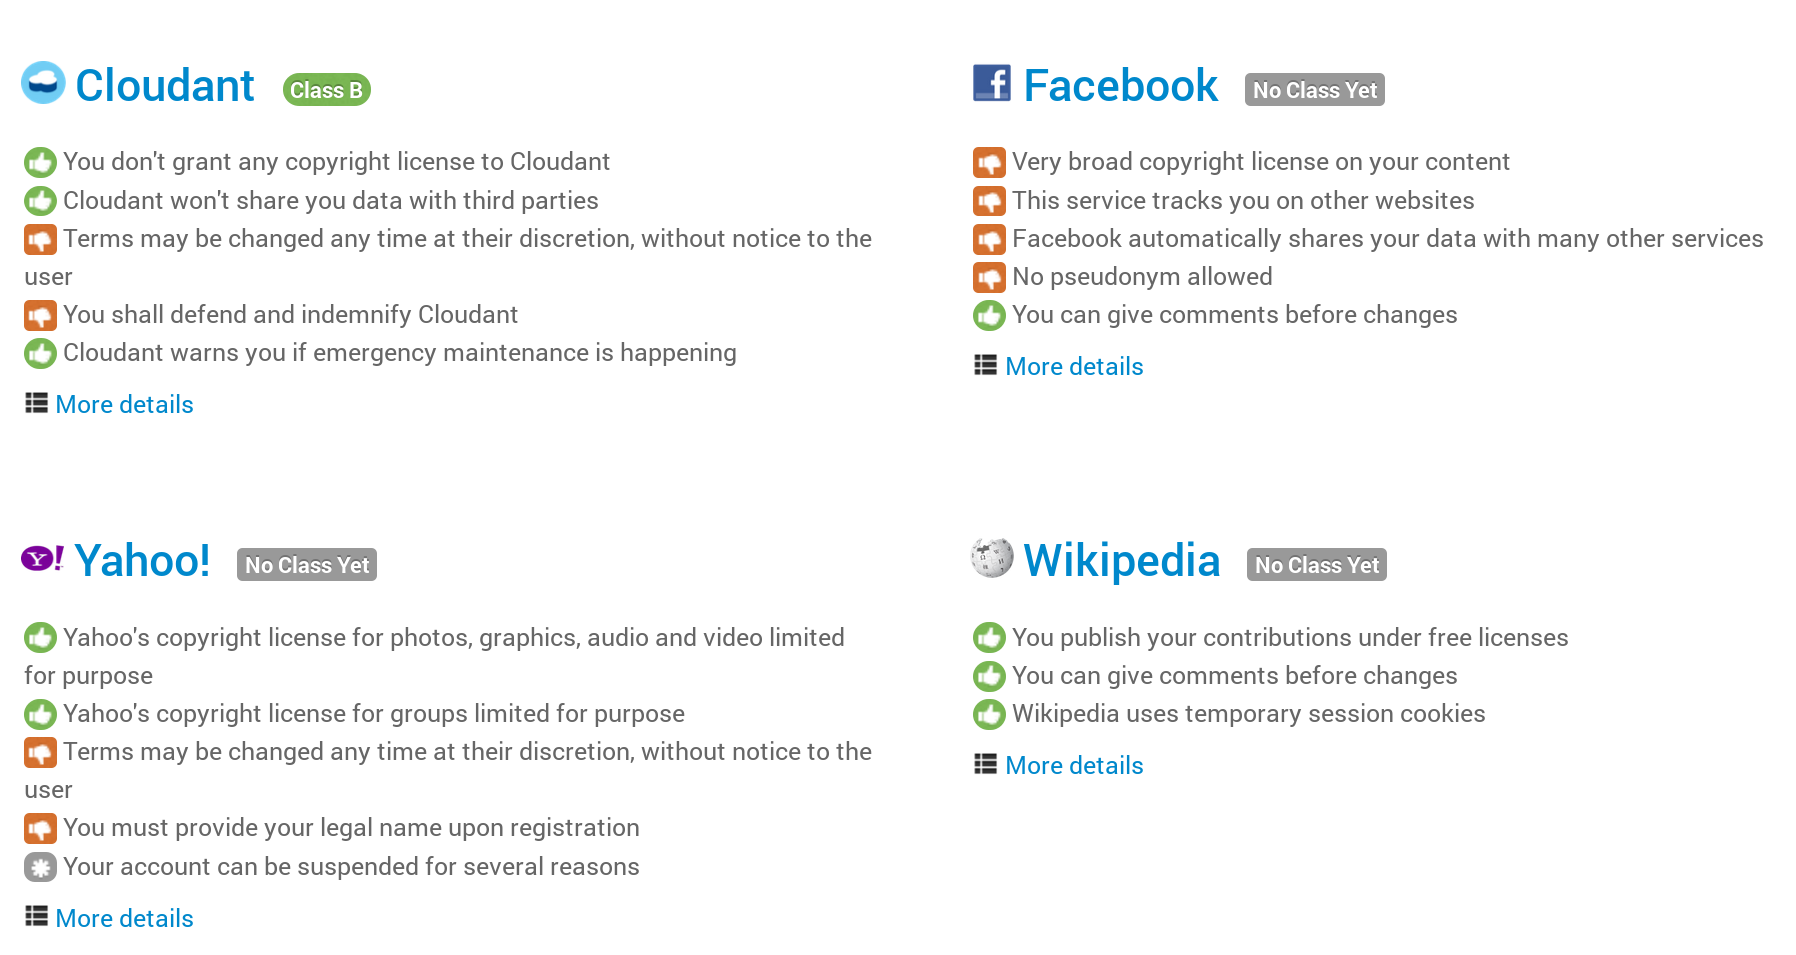
\includegraphics[width=\textwidth,height=\textheight,keepaspectratio]{./tosdr.png} 
\end{frame}
}

\begin{frame}
{More cookies!}
\centering

\includegraphics[width=\textwidth,height=\textheight,keepaspectratio]{./cookie-monster.jpg} 
\end{frame}

\begin{frame}
{Cookie ?}
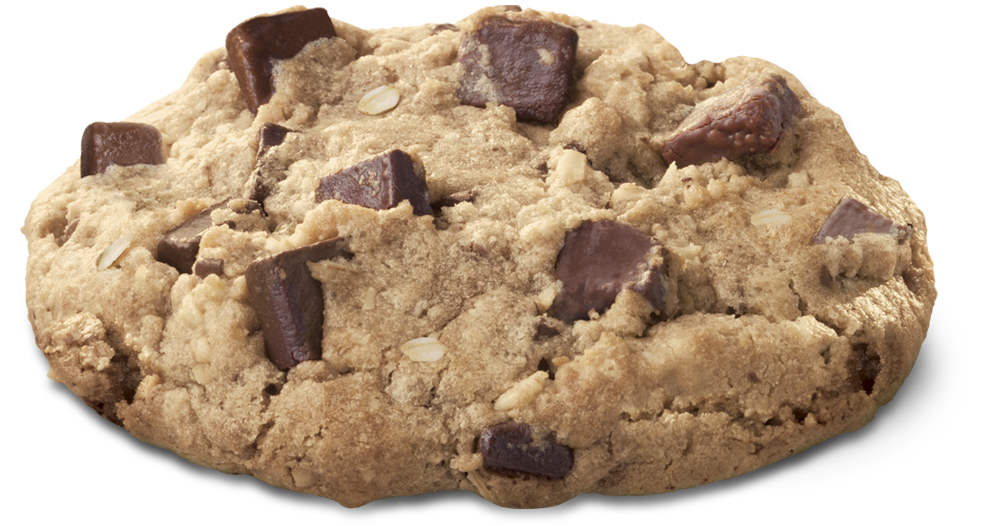
\includegraphics[height=2cm,keepaspectratio]{./cookie.png} 
\newline \newline
Non, pas le gâteau : le fichier-témoin déposé sur votre ordinateur
\end{frame}

\begin{frame}
{Cookie ?}
\centering
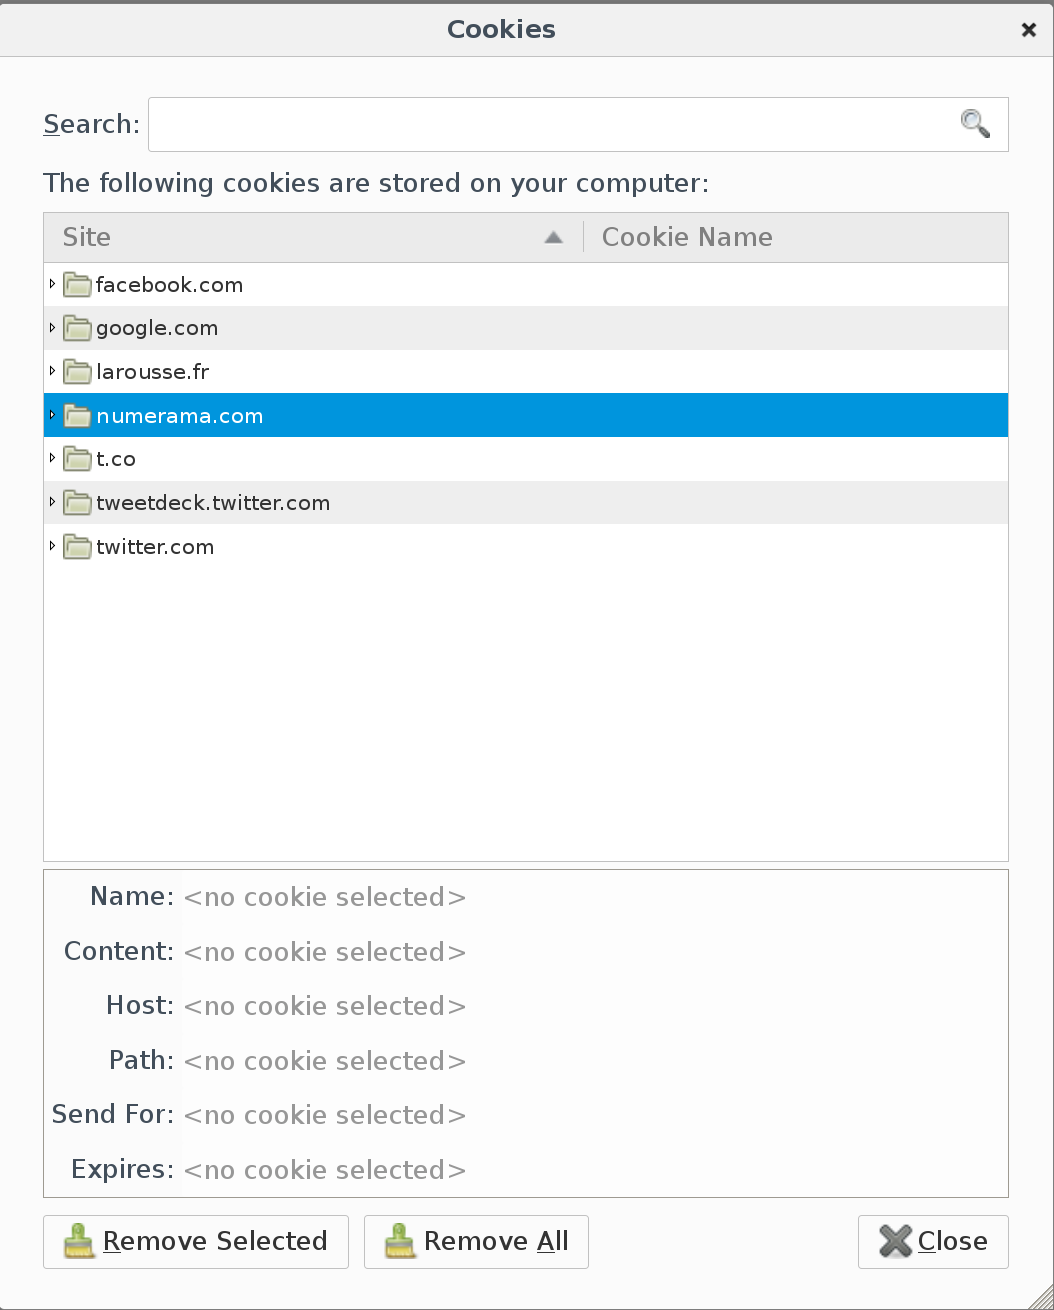
\includegraphics[height=\textheight, width=\textwidth,keepaspectratio]{./cookies.png} 
\end{frame}

\begin{frame}
{Utilisation du cookie}
\begin{itemize}
\item Session (identification auprès du service)
\item Traceur ("like", "g+", "share it", etc)
\item Statistiques
\item Et encore plein-plein de choses
\end{itemize}
\end{frame}

\begin{frame}
{Conclusion}
C'est comme la poussière chez vous : générée principalement par l'occupant, un peu par ses invités.
\newline
\newline
Sauf que chez vous, c'est vous qui passez l'aspirateur*.
\newline
\newline
\textit{* à priori ;)}
\end{frame}

{
\setbeamertemplate{footline}{%
	\begin{beamercolorbox}[wd=\paperwidth,dp=8pt,ht=12pt,leftskip=.29cm,rightskip=.3cm]{linecolor}
	\hfill
	\inserttitle
	\end{beamercolorbox}%
}
{
\centering
\begin{frame}
{Questions ?}

\href{https://ethack.org/}{https://ethack.org/} \\
\vspace{0.3cm}
\href{https://www.twitter.com/EthACK_org}{@EthACK\_org} on Twitter \\
\vspace{0.3cm}
\href{https://www.facebook.com/ethack.org}{ethack.org} on Facebook

\vspace{0.5cm}


\includegraphics[width=4cm]{../common/logo_537.png}
\end{frame}
}
}

\end{document}
